\documentclass{sigchi}

% Use this command to override the default ACM copyright statement (e.g. for preprints). 
% Consult the conference website for the camera-ready copyright statement.


%% EXAMPLE BEGIN -- HOW TO OVERRIDE THE DEFAULT COPYRIGHT STRIP -- (July 22, 2013 - Paul Baumann)
% \toappear{Permission to make digital or hard copies of all or part of this work for personal or classroom use is 	granted without fee provided that copies are not made or distributed for profit or commercial advantage and that copies bear this notice and the full citation on the first page. Copyrights for components of this work owned by others than ACM must be honored. Abstracting with credit is permitted. To copy otherwise, or republish, to post on servers or to redistribute to lists, requires prior specific permission and/or a fee. Request permissions from permissions@acm.org. \\
% {\emph{CHI'14}}, April 26--May 1, 2014, Toronto, Canada. \\
% Copyright \copyright~2014 ACM ISBN/14/04...\$15.00. \\
% DOI string from ACM form confirmation}
%% EXAMPLE END -- HOW TO OVERRIDE THE DEFAULT COPYRIGHT STRIP -- (July 22, 2013 - Paul Baumann)


% Arabic page numbers for submission. 
% Remove this line to eliminate page numbers for the camera ready copy
\pagenumbering{arabic}


% Load basic packages
\usepackage{balance}  % to better equalize the last page
\usepackage{graphics} % for EPS, load graphicx instead
\usepackage{times}    % comment if you want LaTeX's default font
\usepackage{url}      % llt: nicely formatted URLs

% llt: Define a global style for URLs, rather that the default one
\makeatletter
\def\url@leostyle{%
  \@ifundefined{selectfont}{\def\UrlFont{\sf}}{\def\UrlFont{\small\bf\ttfamily}}}
\makeatother
\urlstyle{leo}


% To make various LaTeX processors do the right thing with page size.
\def\pprw{8.5in}
\def\pprh{11in}
\special{papersize=\pprw,\pprh}
\setlength{\paperwidth}{\pprw}
\setlength{\paperheight}{\pprh}
\setlength{\pdfpagewidth}{\pprw}
\setlength{\pdfpageheight}{\pprh}

% Make sure hyperref comes last of your loaded packages, 
% to give it a fighting chance of not being over-written, 
% since its job is to redefine many LaTeX commands.
\usepackage[pdftex]{hyperref}
\hypersetup{
pdftitle={GlassmanUISTDC},
pdfauthor={LaTeX},
pdfkeywords={UIST, DC},
bookmarksnumbered,
pdfstartview={FitH},
colorlinks,
citecolor=black,
filecolor=black,
linkcolor=black,
urlcolor=black,
breaklinks=true,
}

% create a shortcut to typeset table headings
\newcommand\tabhead[1]{\small\textbf{#1}}


% End of preamble. Here it comes the document.
\begin{document}

\title{Interacting with Massive Numbers of Student Solutions}

\numberofauthors{1}
\author{
  \alignauthor Elena L. Glassman\\
    \affaddr{MIT CSAIL}\\
    \email{elg@mit.edu}
}

\maketitle

\begin{abstract}
This is an HCI approach to dealing with multiple solutions generated by students. Many coding problems have a specification that the student's solution must meet, but give the student a broad range of freedom for the internal design of that solution. There may be several distinct, correct solutions, some of which may be unknown to the teaching staff or intelligent tutor designer, making it potentially difficult for staff to help students reach their own correct solutions. My approach is to visualize hundreds or thousands of student solutions to discover alternatives, and classify the solutions through interactive machine learning. The visualization and classifications can inform assistance given to students, in the form of staff-student discussions, peer-pairing, and/or automated help.
\end{abstract}

\keywords{
	Guides; instructions; author's kit; conference publications;
	keywords should be separated by a semi-colon.
	\textcolor{red}{Mandatory section to be included in your final version.}
}

\category{H.5.m.}{Information Interfaces and Presentation (e.g. HCI)}{Miscellaneous}

\section{Introduction}


I build novel user interfaces to improve engineering and programming education when students vastly outnumber their teachers. My contributions are in the field of Human-Computer Interaction (HCI). In order to better support teachers, and their students, I combine techniques from HCI with techniques from machine learning, program analysis, natural language processing, and information visualization.

One example of the challenges I tackle is improving the current state of programming education in a large university course or Massively Open Online Course (MOOC). Many computer programming assignments have a specification that must be met, but give the student a broad range of freedom for the internal design of their solution. There may be several distinct, correct solutions, some of which may be unknown to the teachers. Student-generated solutions are difficult to summarize, explore, and assess. Doing this at scale, where hundreds or thousands of student have submitted a response to the same assignment, is both a challenge and an opportunity. 

Visualization, human-computer interaction, and domain-specific analysis techniques applied to students? solutions at scale will improve the support available to students, provided by staff, peers, and automation. That support can be in the form of (1) tools providing teachers with a new way to explore their students? solutions, (2) websites that help knowledgeable students help peers, or (3) data-driven refinements to automated feedback mechanisms, like auto-graders. I ask the following questions:
How do we help teachers understand the design space of solutions generated by students?
What (a) features of solutions and (b) features in a user interface are useful for visualizing and clustering alternative solutions?
How can students help each other debug and explore alternative designs?

\begin{figure*}[t!]
\centering
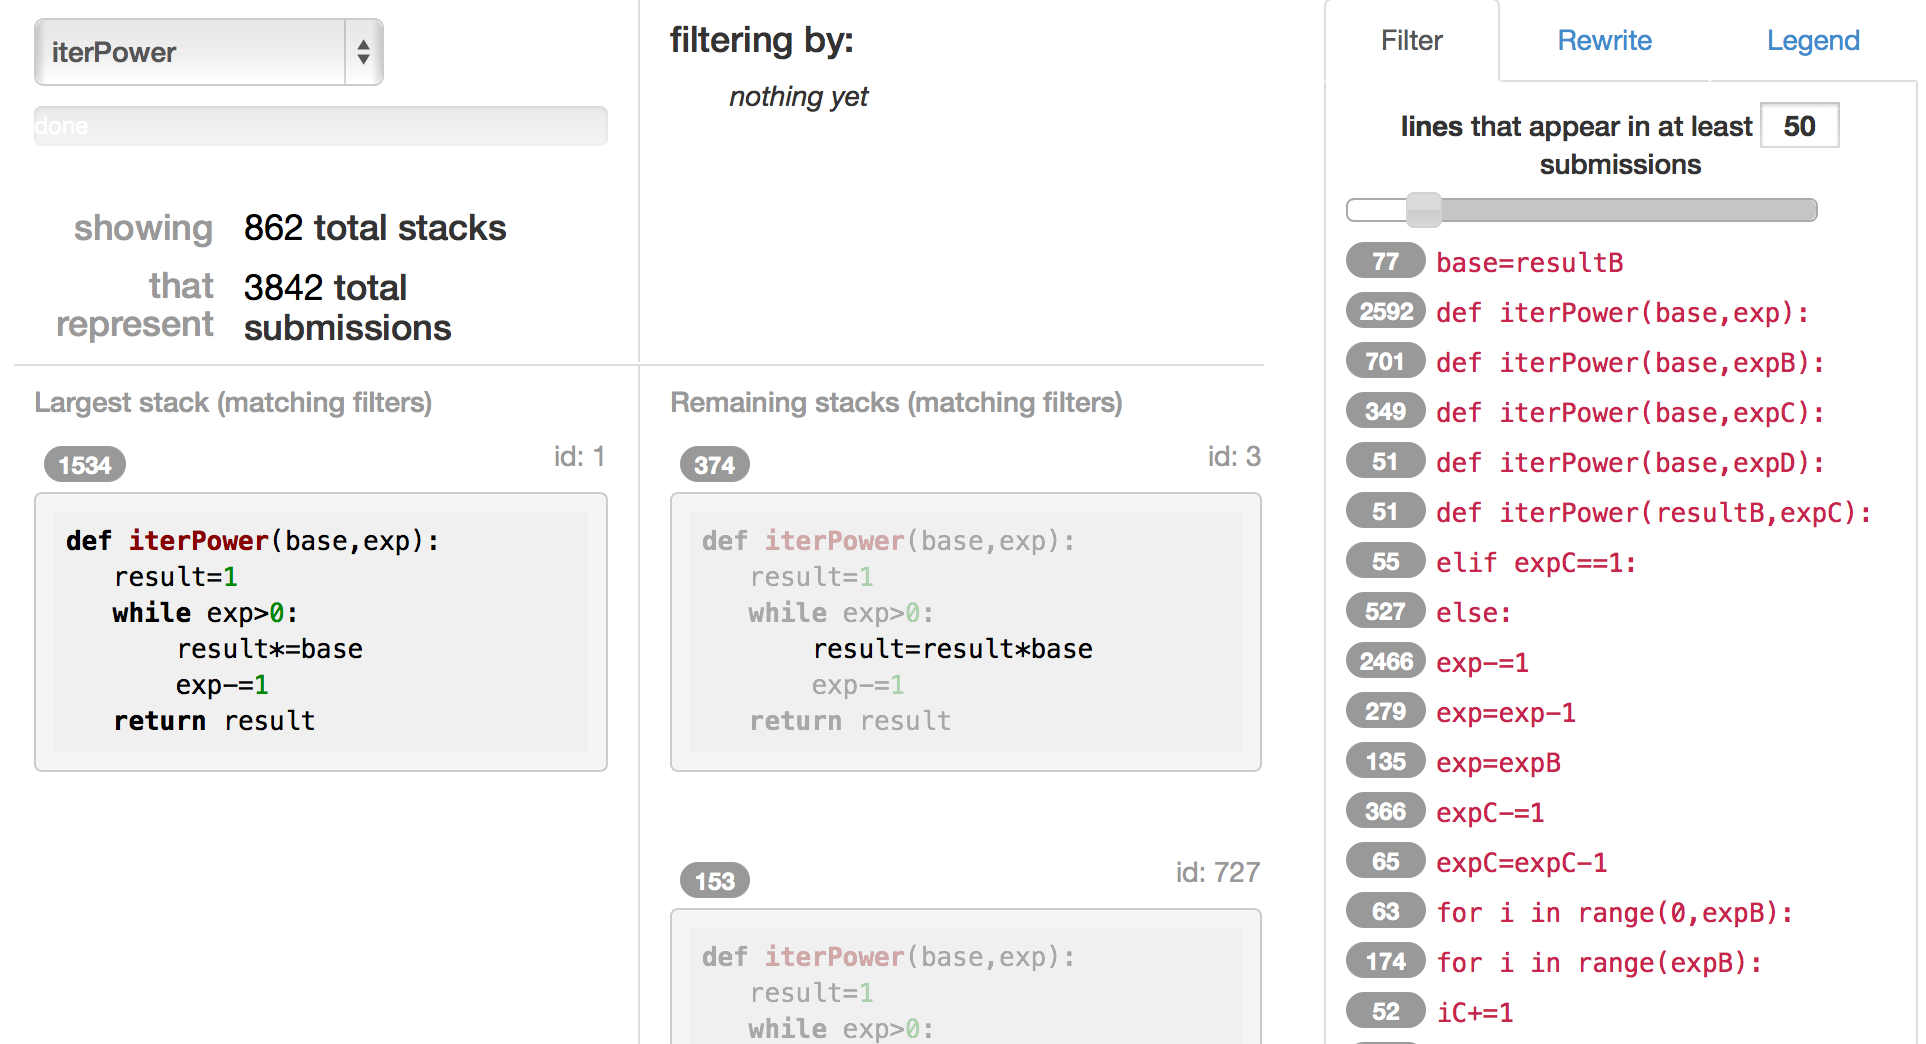
\includegraphics[width=0.9\textwidth]{frontPageInterfacePreview.png}
\caption{OverCode user interface.}
\label{fig:figure1}
\end{figure*}

\section{Visualizing, Clustering, and Exploring Code}
To begin to answer the first and second questions, I led the development of OverCode, a system for visualizing and exploring the variation in hundreds or thousands of programming solutions generated by students attempting a set of Python programming exercises in a large university course or MOOC. Understanding the wide variation in students? solutions is important for providing appropriate, tailored feedback to students, refining evaluation rubrics, and exposing corner cases in automatic grading tests. For example, without tool support, a teacher may not read more than 50-100 solutions before growing frustrated with the tedium of the task. Given a relatively small sample size of the spectrum of solutions, teachers cannot be expected to develop a thorough understanding of the variety of strategies used to solve the problem, or produce instructive feedback that is relevant to a large proportion of learners. They are also less likely to discover unexpected, interesting solutions.

OverCode?s novel backend cleans up student solutions for easier visualization by renaming variables that behave the same across different solutions. With lightweight static analysis after renaming variables, the backend creates clusters of functionally identical solutions. The cleaned solutions are readable, executable, and describe every solution in its cluster. The algorithm?s running time is linear in both the number of solutions and the size of each solution. 

OverCode?s frontend presents the cleaned solutions as each cluster?s unique descriptor, which otherwise would be difficult to automatically generate. In Fig. \ref{fig:figure1}, a, b, and c are cleaned solutions with renamed variables representing clusters of 1534, 374, and 153 solutions, respectively. The differences between clusters (d) are highlighted. Given those initial clusters, OverCode lets teachers further filter (e) and merge (f) clusters based on rewrite rules.

Compared to a non-clustering baseline, OverCode allowed teachers to (1) more quickly develop a high-level view of students? understanding and misconceptions, and (2) plan course forum posts with feedback that is relevant to more students. We are currently extending OverCode?s pipeline to include other languages, such as Java and hardware description languages, and more complex coding assignments. I hope OverCode will help teaching staff continue to get a deeper insight into their students? design choices.


\section{Social System Engineering}
To answer the third question, ``How can students help each other debug and explore alternative designs?'' I am pilot testing various ways for students to help their peers while also benefiting from the process of synthesizing explanations.

\subsection{Evaluating Alternative Designs} In MIT's Computation Structures course, students create digital circuits in a hardware description language. Through exploration of hundreds of previous students? solutions, I found that the space of alternative correct circuit designs is nearly completely separable by the number of device primitives, i.e., transistors, in each design. Picking from previous students? designs, I was able to automatically present current students with design alternatives that were better or worse than their own. Students were asked to give advice to a future student about how to improve the poorer of the two designs. Their explanations gave a rich window into their understanding. Students in the Spring '14 offering of the course gave strikingly cogent advice to future students. How best do we close this loop, so that students benefit from the design alternatives and advice generated by classmates? 

\subsubsection{Incorporating Interactive Visualization}
The interactive Solution Maps in Cody, MathWork's programming game, plot static features of submitted student solutions, such as parse tree size, that can separate students' solutions into clusters \cite{Cody}. They are provided to learners for their potential educational benefit. What changes to OverCode are necessary to create a visualization of fellow students' solutions that is beneficial for students' learning, instead of teachers' understanding?

\subsection{Pairing Students Based on Their Designs} In another assignment in the same course, students are asked to create a Turing machine that determines whether a string of parentheses is balanced, i.e., has a closing parenthesis for every open one. I visualized the dynamic behavior of over a hundred students? Turing machines, and found that there were two distinct common designs. Several fellow teachers were only aware of one. At least one teacher admitted steering students away from designs that, in retrospect, may have been the ?other? common solution they did not know about. In addition to better preparing teachers, can we automatically recognize which design a student is working on? When they need help, should we pair them with another student who is working on, or has already finished, the same design? How do we support, or at least not interfere with, students working toward novel designs?

\subsection{Debugging Advice Based on Test Cases} In the same course, students ultimately build entire simulated processors composed of logic gate primitives. These designs, expressed as pages? worth of an in-house declarative programming language, can become so complex as to be very challenging to debug even with the one-on-one help of a seasoned teaching staff member. Students who have previously resolved a bug can be in a better position than a staff member to help a fellow student with the same bug, if the staff member has never encountered that bug before. 
``Dear Beta'' is a website I built so that students can post explanations of their own resolved bugs, indexed by the failed test cases the bug caused. Providing the explanation is pedagogically useful, and students struggling with a bug can reference it for advice. When students sought help and found one of their fellow students? hints helpful, they had the option of upvoting it. Both website usage statistics and anecdotal evidence, including a student?s unprompted class forum thank you note, suggest that a subset of students find the website to be very helpful. What are the necessary factors to consider when generalizing this peer-helping framework to additional software design courses?

\section{Summary}
At the conclusion of my graduate work, I hope to have built systems that help both teachers and students in engineering and programming courses. In the development process, I hope to describe essential design principles for such systems, and show that teachers using the systems get deeper insight into their students' thoughts and designs, allowing richer conversations with students about their design choices. To better support learners when teachers are vastly outnumbered by students, or when teachers are simply not present, I hope that these systems help students help each other.








\section{Acknowledgments}

This material is based, in part, upon work supported by the National Science Foundation Graduate Research Fellowship (grant 1122374), the Microsoft Research Fellowship, the Bose Foundation Fellowship, and by Quanta Computer as part of the Qmulus Project.  Any opinions, findings, conclusions, or recommendations in this paper are the authors?, and do not necessarily reflect the views of the sponsors.

% Balancing columns in a ref list is a bit of a pain because you
% either use a hack like flushend or balance, or manually insert
% a column break.  http://www.tex.ac.uk/cgi-bin/texfaq2html?label=balance
% multicols doesn't work because we're already in two-column mode,
% and flushend isn't awesome, so I choose balance.  See this
% for more info: http://cs.brown.edu/system/software/latex/doc/balance.pdf
%
% Note that in a perfect world balance wants to be in the first
% column of the last page.
%
% If balance doesn't work for you, you can remove that and
% hard-code a column break into the bbl file right before you
% submit:
%
% http://stackoverflow.com/questions/2149854/how-to-manually-equalize-columns-
% in-an-ieee-paper-if-using-bibtex
%
% Or, just remove \balance and give up on balancing the last page.
%
\balance

\section{References format}
References must be the same font size as other body text.
% REFERENCES FORMAT
% References must be the same font size as other body text.

\bibliographystyle{acm-sigchi}
\bibliography{sample}
\end{document}
